
\section{Preliminary Evaluation}

\label{sec:eval}
\parab{Evaluation Settings}
We use a realistic workload based on a
one-hour Hive/MapReduce trace collected from a Facebook
production cluster \cite{coflow-benchmark}. The trace contains more
than 500 Coflows observed in a datacenter with 150 ToRs.
For the network model, we assume that each ToR has 192 available ports (\ie, $k=192$), which is the case for MegaSwitch \cite{megaswitch}. We set each inter-port connection to carry 1Gbps capacity. %and we set  the reconfiguration delay $\delta$ to 20$ms$.

\begin{figure}[t]
  \centering
  \subfloat[][Traffic distribution within one coflow]{\label{fig:trace01}%
    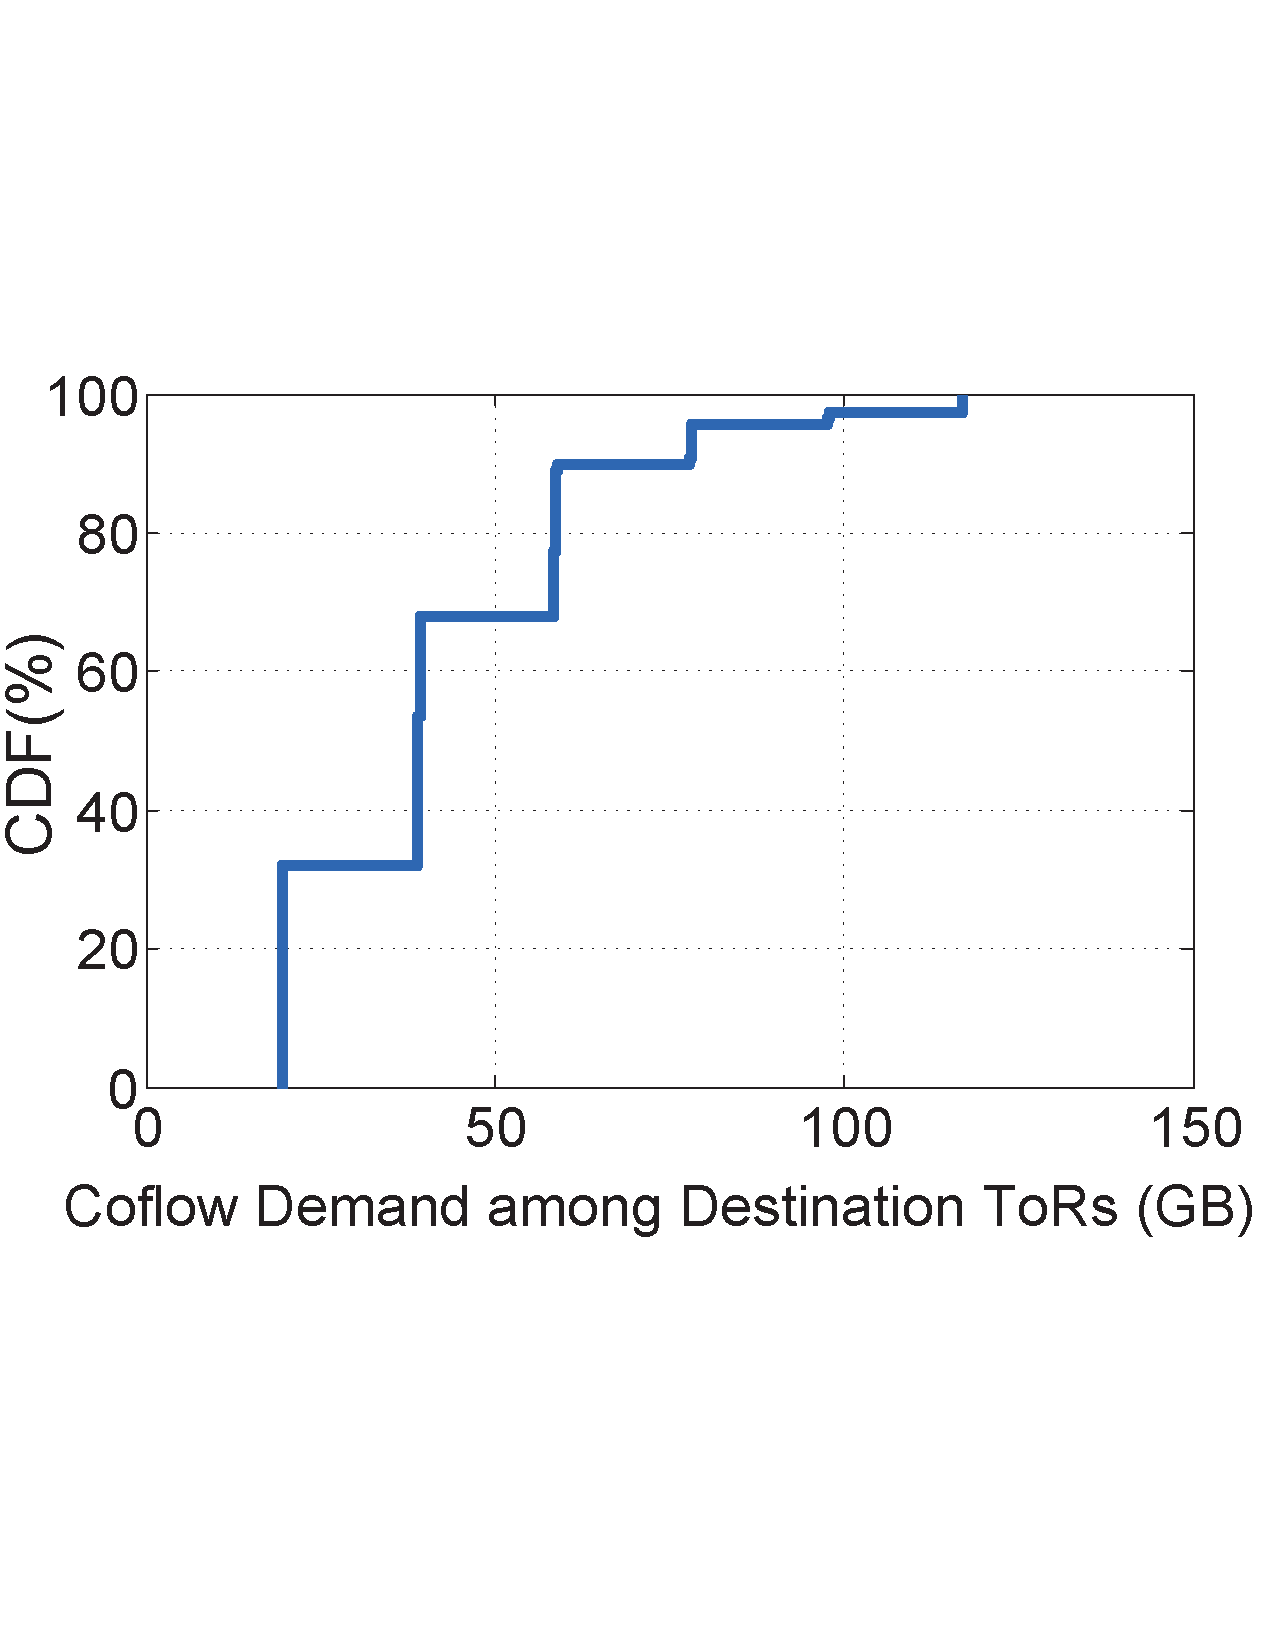
\includegraphics[scale=0.194]{figures/size55}%
  }
\hfill
   \subfloat[][CDF of $\gamma$]{\label{fig:trace02}%
    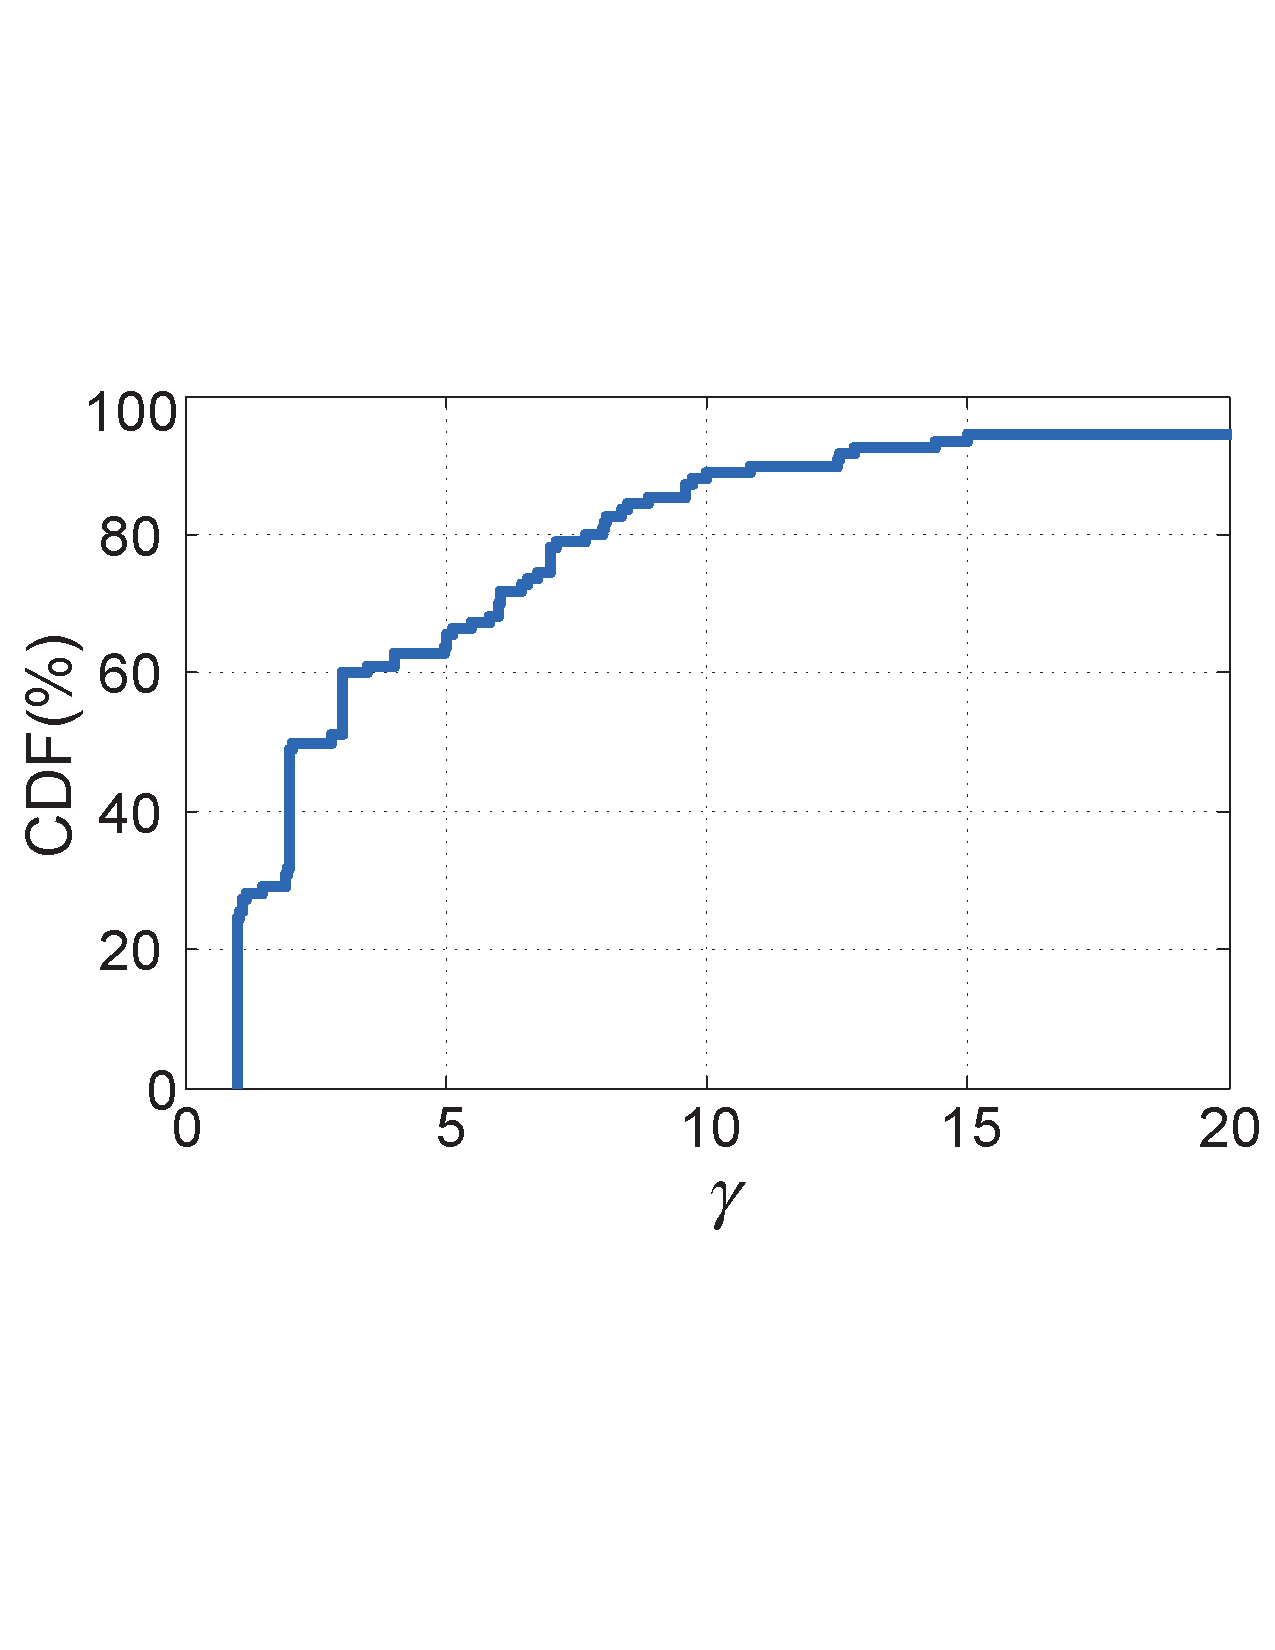
\includegraphics[scale=0.195]{figures/size311}%
  }
  %%\vspace{-0.03in}
  \caption{[Evaluation] Traffic pattern within a coflow can be very biased.}
  \label{fig:trace}
\end{figure}


\parab{Understanding the Coflow Structure}
We first study how the traffic is distributed within a coflow in the Facebook trace. Note that such coflow structure is directly related to the performance of the scheduling algorithm.  For example, in Example \ref{fig:1} if all the flows of coflow $C$  have the same size, then circuit shaping also achieves the optimal CCT.
%In particular, recall that for the circuit shaping algorithm, the inefficiency lies in the mismatch between the circuit configuration and the coflow structure.
%Such mismatch tends to be more severe when the flow size within a coflow follows a biased distribution.
In particular,
the mismatch in circuit shaping tends to be more severe when the flow size within a coflow follows a biased distribution.

Observation from the Facebook trace validates that the traffic pattern within a coflow can be very biased.
To show this, we first select a large coflow with widespread communication among more than 120 ToRs and inspect its structure. Figure \ref{fig:trace01} demonstrates how the traffic is distributed among destination ToRs --- 25\% of the ToRs receive less than 2GB data, while another 25\% receives more than 6GB.

To show that such a coflow is no corner case, we define $\gamma$
as the ratio between the maximum and minimum traffic demand within a coflow among all destination ToRs.
Figure \ref{fig:trace02} shows the distribution of $\gamma$ for all coflows with wide-spread communication pattern\footnote{
Coflows which contain more than 100 subflows with different source and destination.}.
We see that for 40\% of the coflows, some ToR receives 3$\times$ data compared to some others.
And 20\% of the coflows experience a larger bias of 8$\times$.


\parab{Effectiveness of Joint Shaping}
We implement a flow-level simulator to evaluate the effectiveness of the joint shaping heuristic in the simplified single coflow case. We evaluate three algorithms: the optimal solution (calculated by Equation \ref{equ:2}), the circuit shaping and the joint shaping. For easy comparison, we normalize
the achieved CCT of circuit shaping and joint shaping over the optimal solution, \ie,
\begin{equation*}
%\begin{small}
\text{Normalized Comp. Time} = \frac{\text{Compared CCT}}{\text{Optimal CCT}}
%\end{small}
\end{equation*}
Smaller values indicate better performance, and a normalized completion time close to 1 indicates comparable performance to the optimal solution.



Figure \ref{fig:result} presents comparative CDFs of CCTs for
all coflows with wide-spread communication patterns.
We first notice that circuit shaping performs poorly compared to the optimal solution. In particular, 40\% of the coflows finish 1.6$\times$ slower than the optimal.
This is because under the biased coflow structure, the mismatch between the circuit configuration and the coflow structure becomes severe. Note that the performance of circuit shaping is also the best achievable performance for all algorithms with direct routing (\eg, Sunflow \cite{sunflow}, Solstice \cite{solstice}) under our evaluation settings.

\begin{figure}[t]
  \centering
  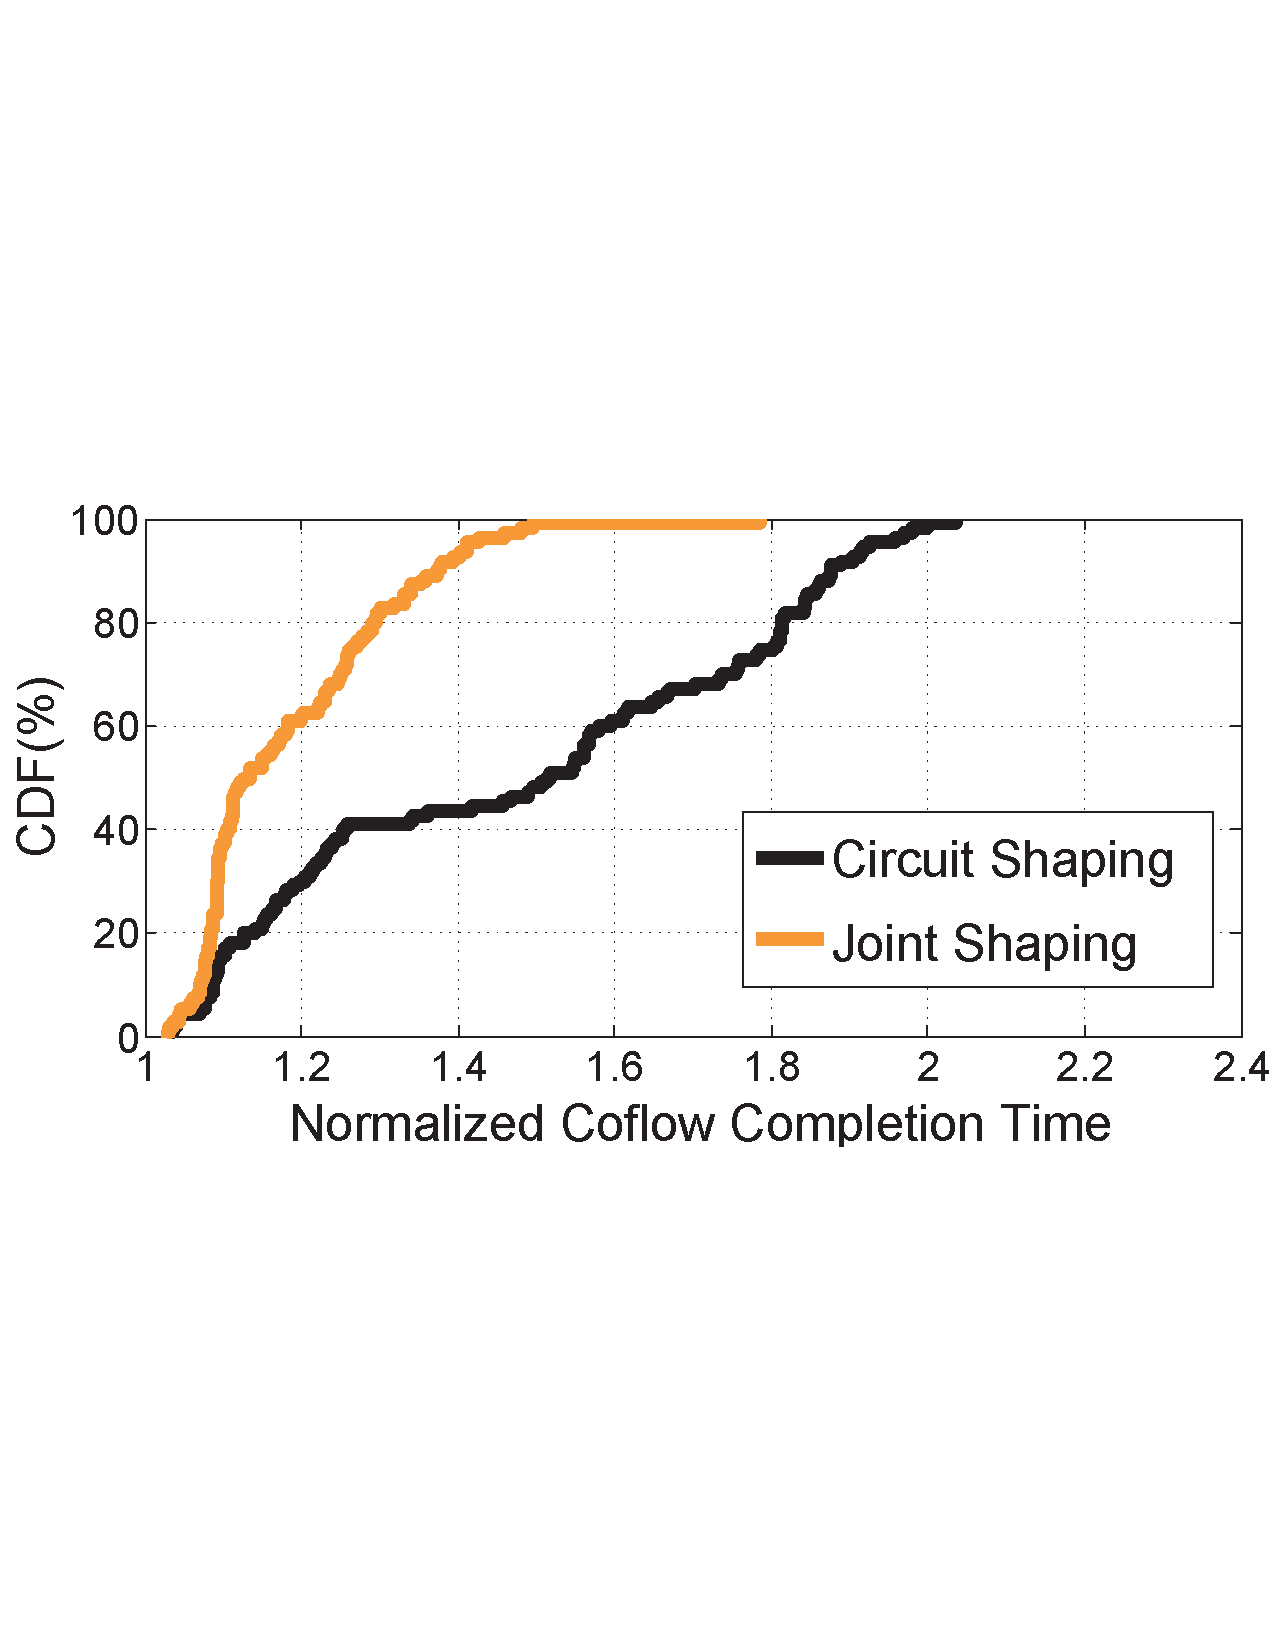
\includegraphics[scale=0.32]{figures/initial1}%
  \caption{[Evaluation] CDF of the normalized CCT. We see that joint shaping significantly outperforms the circuit shaping algorithm.}
  \label{fig:result}
\end{figure}

Moreover, we observe that the simple heuristic (Algorithm \ref{ALG-1}) for joint shaping approaches the optimal solution, and significantly outperforms the circuit shaping algorithm. Specially, 40\% of the coflows finish within 1.1$\times$ of the optimal, and 80\% are within 1.3$\times$.
We also calculate the average normalized CCT. The result shows that joint shaping is within 1.18$\times$ to optimal, and outperforms circuit shaping by 30\%.

%\parab{Remark} Evaluation of the general case is left as future work.
%Evaluation with production trace show that such mismatch is no corner case, which enlarges the CCT by over $40\%$ in average.



